\chapter{RC and RL Transient Signals}


\section{Introduction}

In this lab you will use explore transient behavior of$RC$ and $RL$ circuits.  You will learn
how to use scope probes and measure properties of waveforms on your digital oscilloscope using cursors.  For this lab there are both logbook and jupyter notebook entries.


%\section{Pre-lab Calculation}
%
%\noindent
%1) Show that for an exponential decay with time constant $\tau$, the rise-time, when defined as the time interval between $10\%$ and $90\%$ values, is given by:
%\begin{displaymath}
%t_{90} = {\rm ln}(9) \; \tau \sim 2.2 \; \tau
%\end{displaymath}
%
%\noindent
%2) Calculate the inductance of a solenoid with N=20 turns, length $\ell=4~\rm cm$, a radius of $1~\rm cm^2$ using the formula:
%\begin{displaymath}
%L = \frac{\mu_0 N^2 A}{\ell}
%\end{displaymath}
%where $A$ is the cross-sectional area and $\mu_0 = 1.257 \times 10^{-6}~\rm H/m$.


\section{Transient Response of an $RC$ Circuit}

\begin{figure}[htbp]
\begin{center}
\begin{tikzpicture}
    \node[anchor=south west,inner sep=0] (image) at (0,0,0)
         {\includegraphics[height=0.30\textheight]{figs/labs/transients/probe_setup.jpg}};
         \node[left](X) at (-1.0,4.0) {Probe Tip}; \draw (X.east) --
         (5.0,2.4); \node[left](X) at (-1.0,3.0) {Ground Clip}; \draw
         (X.east) -- (5.4,2.2); \node[right](X) at (10.0,5.0) {BNC
           Tee}; \draw (X.west) -- (8.0,5.2); \node[right](X) at
         (10.0,4.0) {Alligator pair}; \draw (X.west) -- (6.5,2.8);
\end{tikzpicture}
\caption{A setup for connecting the scope probe directly to the output of the function generator.}
\label{fig:probe_setup}
\end{center}
\end{figure}

Set your Channel 1 of your function generator to produce Square wave
output with a peak-to-peak voltage of $6~\rm V$ and a frequency of
$1~\rm kHz$.  As shown in Fig.~\ref{fig:probe_setup}, use a BNC Tee adapter
to split the output into two copies.  Send one copy directly to the
Channel 1 input of your scope.  Send the other copy to a
BNC-alligator-pair cable.  

Install an oscilloscope probe at Channel 2 of your scope (see Fig~\ref{fig:probe}).  Some probes
in the lab have the ability to switch between attenuation factors near
the probe tip.  If you have such a probe, select the 10X setting.  The
remaining probes have a fixed attenuation of 10X.

So far, we haven't had to worry about proper grounding procedure,
because this is automatically handled by the BNC cable.  Your scope
probe has two main parts, the larger probe tip, which slides to reveal
a hook which can be attached to wires and components in your circuit,
and a short lead ending with a black alligator clip called the
``Grounding clip''.  Handheld devices like your DMM have no connection
to earth ground.  The voltage reference point at the Common terminal
can be connected anywhere you would like in a circuit.  Your scope is
quite different!  It plugs into a wall outlet for power and is
referenced to earth ground.  To provide a scope which is both safe and
cost effective, most scopes are limited to making measurements which
are referenced to ground when using ordinary probes.  The ground clip
of your scope can only be connected to earth ground.  If you connect
it anywhere else in your circuit, that part of your circuit will be
short-circuited to ground.

For now, connect the probe directly to the output of the
function generator.  Your function generator is also referenced to
earth ground.  In particular for this setup, the black alligator clip
is earth ground.  Connect the black clip from the function generator
to the grounding clip for the scope probe.  Next connect the scope
probe to the red alligator clip from the function generator.  You now
have two copies of the function generator output being sent to the
scope.  One directly through the BNC cable, and one through a 10X
attenuation scope probe.

Adjust your scope to view the function generator output as measured by
Trigger 1.  Set the voltage scale as large as possible while observing
the entire wave form.  Leave the timescale at the default setting of
$500~\mu s$ for now.  Check that trigger is on the Falling edge, as set
in the last section.  Set the trigger near threshold near 0 volts.
You should observe that the position of the waveform does not vary
much with trigger threshold: the steep falling edge of the square wave
function gives us a solid reference point for defining $t=0$ in the
measurements that follow.

Now enable Channel 2 on your scope. Adjust all the necessary setting for Channel 2. It should be an identical copy of
Channel 1.  Too see both channels at the same time, you'll have to
move the vertical position of Channel 1 slightly. Closed loop tests
like this are the way experienced scientists and engineers always
start.  It allows you to setup your signal generator and scope
properly, without adding the complexity of the circuit you are working
on.  In general, avoiding confusion by taking small incremental steps
is the fastest, most reliable way to proceed in lab.  

\begin{figure}[htbp]
\begin{center}
\begin{tabular}{cc}
\begin{circuitikz}[line width=1pt]
\draw (0,0) to[square voltage source,bipoles/length=1.5cm] ++(0,4.0) to[short] ++(2.0,0)
to[R,-*] ++(0,-2.0) coordinate(X) to[short,*-o] ++(1.0,0) node[right]{A};
\draw (X) to[C,-*] ++(0,-2.0) coordinate(X) to[short,-o] ++(1.0,0) node[right]{B};
\draw (X) to[short,-*] ++(-2.0,0) node[ground,yscale=2.0]{};
\end{circuitikz}  &
\begin{circuitikz}[line width=1pt]
\draw (0,0) to[square voltage source,bipoles/length=1.5cm] ++(0,4.0) to[short] ++(2.0,0)
to[R,-*] ++(0,-2.0) coordinate(X) to[short,*-o] ++(1.0,0) node[right]{A};
\draw (X) to[L,-*] ++(0,-2.0) coordinate(X) to[short,-o] ++(1.0,0) node[right]{B};
\draw (X) to[short,-*] ++(-2.0,0) node[ground,yscale=2.0]{};
\end{circuitikz}  \\
(a) & (b) \\
\end{tabular}
\caption{A function generator driving an (a) RC circuit, and (b) RL circuit.}
\label{fig:rlc-circuits}
\end{center}
\end{figure}


Construct the circuit in Fig.~\ref{fig:rlc-circuits}a on your
breadboard, as shown in Fig.~\ref{fig:rc_setup}a.  Use $C=10~\rm nF$
capacitor and $R=10~\rm k\Omega$.  
\begin{measurement} Using the given values of resistor and capacitor, calculate and record in your logbook the time constant of the RC circuit  together with its minimum and maximum value assuming 5\% tolerance. Take care to include proper units. Using your DMM, measure and record
the actual resistance and capacitance of your components before
installing them. Record each value together with accuracy of your DMM for that specific measurement (see table~\ref{tbl:accuracy}). Then calculate the time constant of the RC circuit using the measured values. We still did not learn how to propagate uncertainties. Estimate which fractional uncertainty ($\mbox{accuracy of a value}/\mbox{measured value}$) is larger and apply this fractional uncertainty to your calculated time constant. Do the ranges for the estimates of time constant overlap? Add a comment in your logbook. \end{measurement}

 Use your function generator as the square wave
voltage source.  Recall that the black alligator clip is earth ground.
The red alligator clip is the square wave output relative to earth
ground, and corresponds to the upper terminal of the voltage source in
the diagram.  The only valid place to connect the grounding clip of
your scope probe is to earth ground, so connect that to point B in
your circuit.  Connect the scope probe tip to point A.  As shown in
the Fig.~\ref{fig:rc_setup}b, each time the square wave changes
polarity, the capacitor beings charging or discharging until it
reaches equilibrium with the new voltage, revealing the characteristic
exponential transient response.

\begin{figure}[htbp]
\begin{center}
\begin{tabular}{cc}
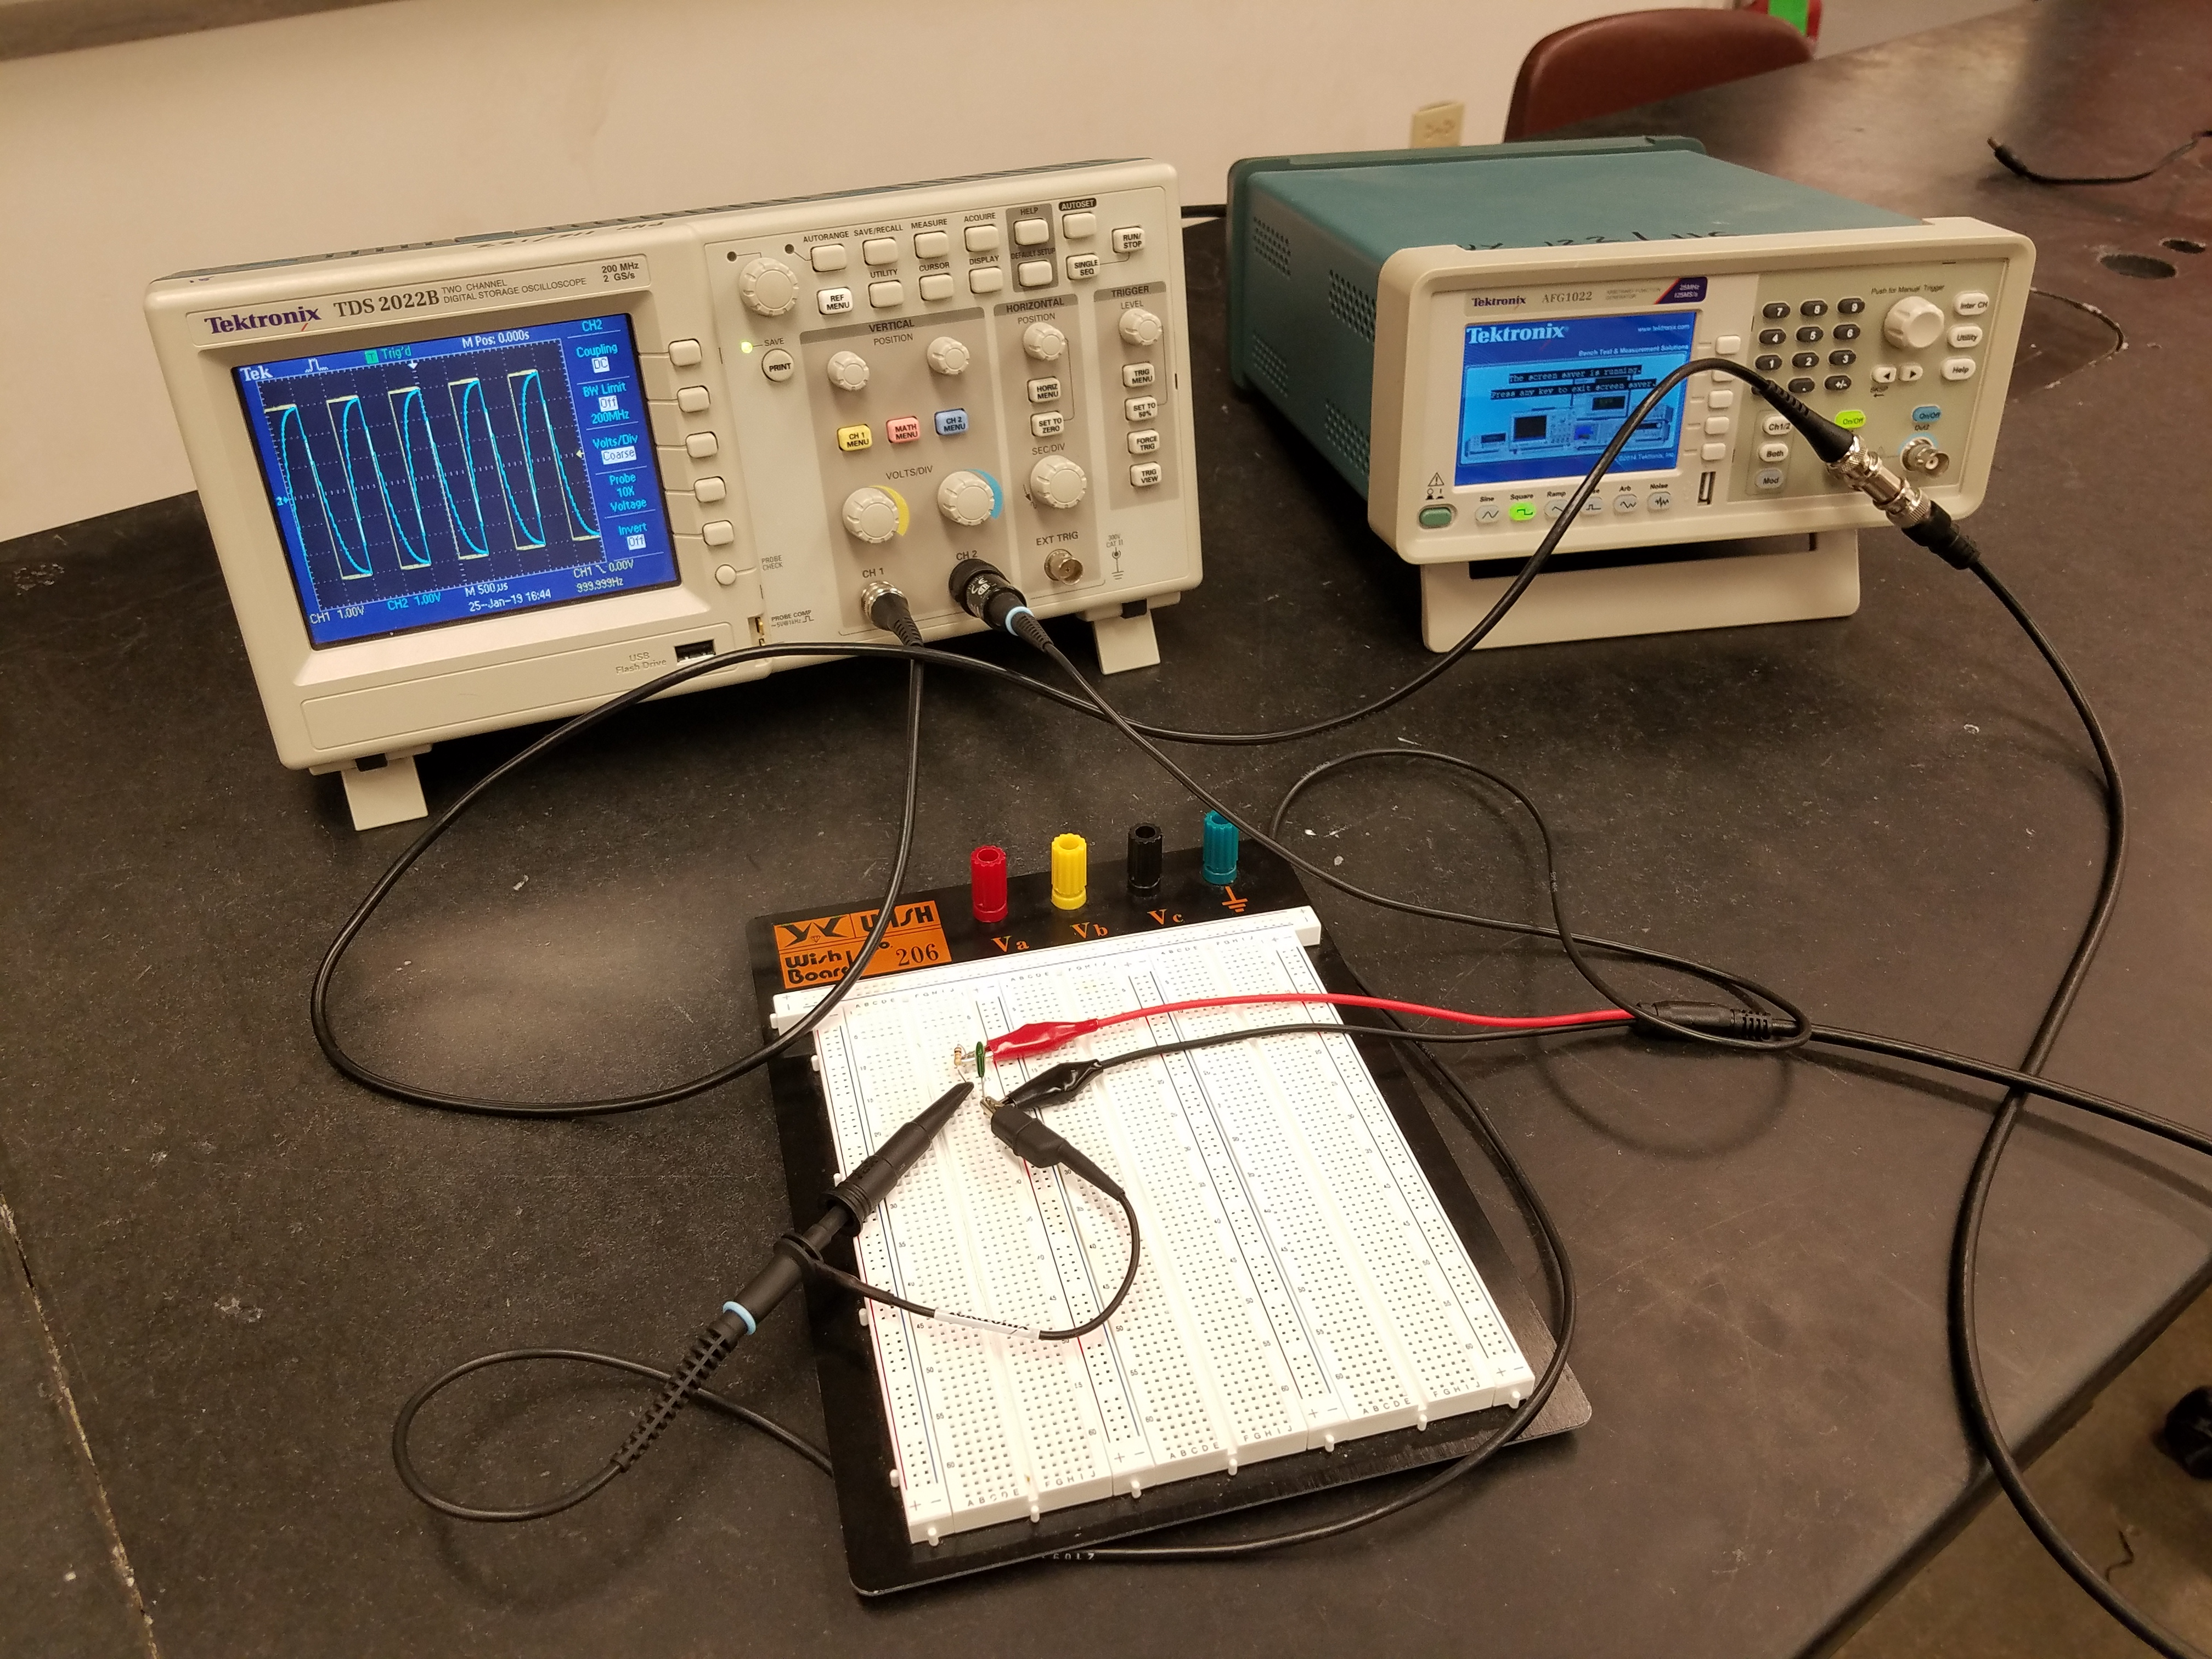
\includegraphics[width=0.45\textwidth]{figs/labs/transients/rc_setup.jpg} &
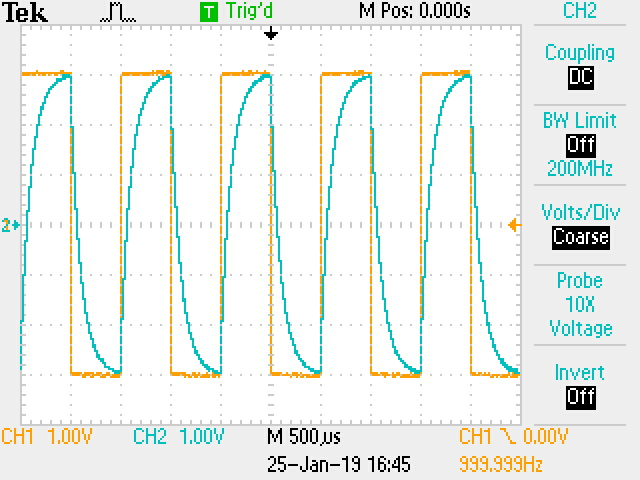
\includegraphics[width=0.45\textwidth]{figs/labs/transients/rc_trace.jpg} \\
(a) & (b) \\
\end{tabular}
\caption{Setup for the (a) RC circuit measurement, and (b) example scope trace showing exponential curve.}
\label{fig:rc_setup}
\end{center}
\end{figure}

\begin{figure}[htbp]
\begin{center}
\begin{tabular}{cc}
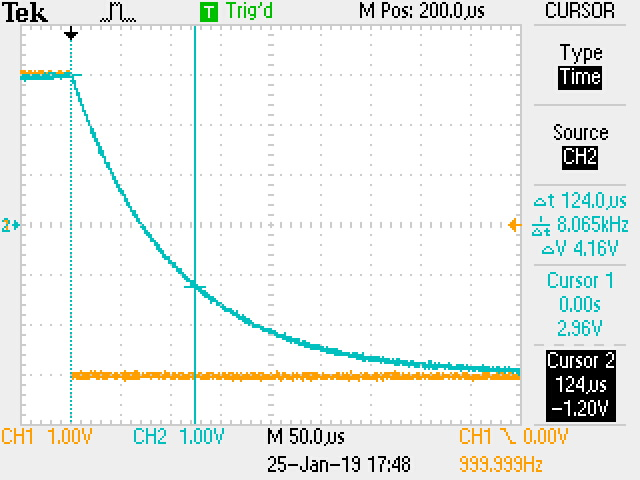
\includegraphics[width=0.45\textwidth]{figs/labs/transients/rc_cursor.jpg} &
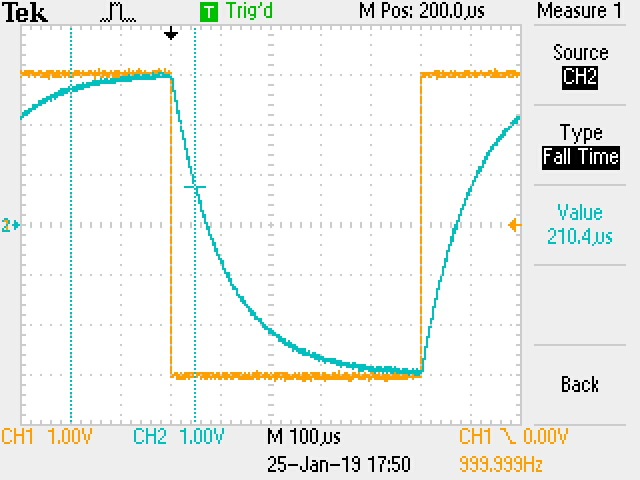
\includegraphics[width=0.45\textwidth]{figs/labs/transients/rc_falltime.jpg} \\
(a) & (b) \\
\end{tabular}
\caption{Scope traces showing (a) use of cursor to measure the waveform at $t=124~\rm \mu s$ and $V=-1.20~\rm V$, (b) use of the built in fall time measurement.}
\label{fig:cursor_falltime}
\end{center}
\end{figure}

Now adjust the timescale to zoom in on the exponential decay portion
of the curve, making sure to keep the trigger position at the left
side of the display, as shown in Fig.~\ref{fig:cursor_falltime}a.
Press the Cursor button, then set Type to Time, and Source to CH2.
This feature allows you to make measurements of different points along
the curve.  Leave Cursor 1 located at $t=0$.  Highlight Cursor 2, by
pressing the corresponding menu button, and adjust it's position using
the multipurpose knob.  Now you can make accurate measurements of the
waveform by reading off the voltage and time at anywhere that you
place the cursor.  
\begin{measurement} Record one measurement every $\sim 25~\rm \mu s$
starting from $t=0~\mu s$ to $400~\rm \mu s$.  (Recall that when
making measurements at target values, you need not hit the target
value exactly, simply record the actual position at which you made
your measurement.) Record also the sketch of your setup and the rough sketch of your waveform.\end{measurement}

\begin{measurement} Your scope can also directly measure the fall time of a waveform.
Setup the function so that one complete falling edge is on screen, as
shown in Fig.~\ref{fig:cursor_falltime}b.  Press Measure and then set
source to CH2 and Type to ``Fall Time''. You might see this value fluctuating. Record five measurements of this value in your logbook.\end{measurement}


\begin{measurement}
Show in your logbook that for an exponential decay with time constant $\tau$, the rise-time, when defined as the time interval between $10\%$ and $90\%$ values, is given by:
\begin{displaymath}
t_{90} = {\rm ln}(9) \; \tau \sim 2.2 \; \tau
\end{displaymath}
\end{measurement}

\begin{plot} Using the above relation and five measurements of fall time calculate the mean value of the time constant of the RC circuit. Recall you can use numpy functions. Calculate also the standard error of the mean value as following: $\sigma_{mean}= \mbox{standard deviation}/\sqrt{\mbox{number of measurements}}$.
\end{plot} 

\begin{measurement} Record the third estimate for the time constant of the RC circuit together with uncertainty in your logbook. Examine now all three different estimates. Are they consistent? Do the ranges for the three estimates of the time constant overlap? Add comment in your logbook about how those estimates compare to each other. Also record your qualitative understanding of this comparison. 
\end{measurement}


% Check that the measured fall time is consistent with your measured values of $R$ and $C$, using the formula from prelab. 


\section{Analysis}

\begin{plot} Plot your collected $RC$ circuit exponential decay data as discrete
data points and compare with the expected exponential decay function
as a continuous curve using the expected $RC$ time constant calculated
from: 1) given value of $R$ and $L$ (Prediction 1), 2) your measured value of $R$ and $L$ (Prediction 2) and 3) your measured value of the fall time via scope (Prediction 3).  Make sure to have
appropriate axis labels and a legend indicating ``Data'',``Prediction 1'', "Prediction 2" and "Prediction 3". 
Describe (in your jupyter notebook) how those predictions are matching your measured data? Could you tell which prediction describes your data best?
\end{plot}

\begin{plot} Redo the plot (in a new inline plot) using a log scale with base of 10 in y axis. To apply logarithmic scale explore the options for plotting in python. A logarithmic scale is a nonlinear scale often used to represent a large range of positive values. You will have to make your voltage measurements larger than zero and you can do this by shifting the measured values by a constant factor. On a logarithmic scale each increment on the axis increases by a factor of 10. On a linear scale each increment on the axis increases by equal fixed increment.  
On a linear scale, a change between two values is perceived as the difference between the values. For example, a change from 1 to 2 is the same amount of increase as from 99 to 100. On a logarithmic scale, a change between two values is perceived as the ratio of the two values. For example, a change from 1 to 2 (ratio of 1:2) is the same amount of increase as a change from 50 to 100 (also a ratio of 1:2). Describe (in your jupyter notebook) how those predictions are matching your measured data? Could you tell which prediction describes your data best? Is this plot more informative? Add these comments to your jupyter notebook. 
\end{plot}

\begin{plot} Plot a difference between data and different prediction as data points in a separate plot. This is so called residual plot. Make sure to have appropriate axis labels and a legend indicating ``Data - Prediction 1'',``Data - Prediction 2'', "Data - Prediction 3".  Recall that you will have to cast your predictions in arrays. Describe (in your jupyter notebook)  how those predictions are matching your measured data? Could you tell which prediction describes your data best? Is this plot more informative? Add these comments to your jupyter notebook. 
\end{plot}



\noindent
This is a \textbf{sign-off point} for this lab. 

\section{Transient response of an RL circuit}


\begin{measurement}
Calculate the inductance of a solenoid with N=20 turns, length $\ell=4~\rm cm$, a radius of $1~\rm cm^2$ using the formula:
\begin{displaymath}
L = \frac{\mu_0 N^2 A}{\ell}
\end{displaymath}
where $A$ is the cross-sectional area and $\mu_0 = 1.257 \times 10^{-6}~\rm H/m$.
\end{measurement}

\begin{measurement}
Wrap an inductor around the provided wooden dowel. Estimate it's
inductance by modifying your calculation above accordingly and record the value in your logbook.  Using your DMM, measure and record the actual resistance. You can skip to estimate accuracy for this measurement.
\end{measurement}


\noindent Turn down the supply to $2.5~\rm V$ peak-to-peak.  Build the circuit in
Fig.~\ref{fig:rlc-circuits}b using your homemade inductor and a
resistor of $R=47~\rm Ohms.$ 
\begin{measurement}
Measure the fall-time of your R-L circuit
and use it to determine a measured value for the inductance.
Determine and record the inductance of your coil and compare to your theoretical
estimate. Add a comment in your logbook. 
\end{measurement}
